% Kapitel 8 - Diskussion
%\clearpage
\section{QFD \& Algorithm Selection}\label{sec:Algorithm definition}

This thesis studies different approaches to develop the algorithm to achieve data reduction. In this chapter different approaches to achieve data compression would be analysed. Also, QFD is a useful tool to define and analyse the requirements and consequently derive an appropriate solution to the problem in the form of an algorithm. The following sub-chapters discuss different approaches to achieve data reduction along with methods like pairwise comparison and weighted analysis used to determine the most optimal approach of all.

\subsection{Mathematical Reduction}\label{sec:Mathematical reduction}
%\ref{datalog}
As mentioned in previous chapters, the existing implementation is focused primarily on the down-sampling of data-stream. Thereafter, the average of each sample is calculated and then stored. While this is not a broken approach, there is a good amount of room for improvement here. While down-sampling with active monitoring for error free sample is a good approach, the existing method has a multi-step approach to achieving the down-sampling and then averaging the results. This approach would be computationally demanding than regular data log generation, as it undergoes a 3 step monitoring process before settling down on the pre-selected sampling frequency to down-sample the data-stream. This would require relatively more time also, naturally, than simple data-log generation. 

Since the logs consists of numerical values, primarily, mathematical approaches for reducing the size of data can definitely not be ignored or discarded. Statistical methods like mean, median, standard deviation or variance could be utilized here since all of them deal with condensing chunks of data into singular or smaller meaningful arithmetic numerals. A quick explanation and summarising of different statistical approaches is hence needed. 

The first method of mean is of particular interest here. The method of mean involves in finding the averages of values and condensing a larger set of value into singular or smaller sets of data that indicate the central tendency. There are several kinds of mean in mathematics, especially in statistics. Each mean serves to summarize a given group of data, often to better understand the overall value (magnitude and sign) of a given data set. For a data set, the arithmetic mean, also known as "arithmetic average", is a measure of central tendency of a finite set of numbers: specifically, the sum of the values divided by the number of values. The arithmetic mean of a set of numbers x1, x2, ..., xn is typically denoted using an overhead bar, $\bar{x}$. \cite{mean} 

There are primarily three types of means that are generally used in statistics. They are as follows: 

\begin{itemize}
    \item Arithmetic Mean
    \item Geometric Mean
    \item Harmonic Mean
\end{itemize}

\textbf{Arithmetic Mean} : also known as the average, is a statistical measure that is used to determine the central tendency of a set of numerical data. The arithmetic mean is calculated by summing all of the values in a data-set and dividing the total by the number of values in the data-set. The arithmetic mean is commonly used in many different fields and is one of the most widely used statistical measures. It is particularly useful in situations where the distribution of data is symmetric and the data is not skewed. It is easy to calculate, easy to understand and is useful in many different types of analyses.  One of the main advantages is that it is easy to understand and calculate. Because the arithmetic mean is based on the sum of all values in a data-set and the number of values in the data-set, it is easy to compute and understand the results. However, there are also some limitations to using the arithmetic mean. One of the main cons is that it can be affected by outliers or extreme values in the data-set. For example, if there is a single extremely large value in a data-set, it can skew the overall mean and make it unrepresentative of the majority of the data. Additionally, the arithmetic mean is not useful for data-sets with skewed distributions, such as those with a lot of small values and a few large values.

The below equation shows how arithmetic mean is calculated : 

\begin{equation}
\bar{x} = \frac{x1 + x2 + x3 + ... + xn}{n}\
\end{equation}

\textbf{Geometric mean} :   is a measure of central tendency that is used to find the average value of a set of numbers by multiplying them together and taking the nth root, where n is the number of numbers in the set. It is often used when working with data sets that have skewed distributions, such as when dealing with exponential growth or decay. One of the main areas of implementation for the geometric mean is in finance and economics, where it is used to calculate the average rate of return on an investment over a period of time. This is particularly useful when comparing investments with different volatility levels, as it gives a more accurate picture of the overall performance of the investment. The geometric mean has some advantages over other measures of central tendency such as the arithmetic mean. It is less sensitive to outliers and extreme values, which makes it a better measure of central tendency when working with skewed data. However, the geometric mean also has some downsides, such as it is not defined for negative values, and it is also not defined for data-sets that contain zero or negative numbers. 

Additionally, it can be difficult to interpret the geometric mean when working with large numbers, as it can be difficult to understand the meaning of the nth root of a large product. In conclusion, the geometric mean is a useful measure of central tendency that is particularly well-suited for data sets that have skewed distributions, and is widely used in finance and economics, statistics and research, it may be not appropriate for data-sets containing negative numbers and it can be difficult to interpret large values. Geometric mean is represented as below :

\begin{equation}
    \left(\prod _{i=1}^{n}x_{i}\right)^{\frac {1}{n}}={\sqrt[{n}]{x_{1}x_{2}\cdots x_{n}}}
\end{equation}


\textbf{Harmonic Mean} :  a type of average that is commonly used to calculate the average of rates or ratios. It is calculated by taking the reciprocal of the arithmetic mean of the reciprocals of the given numbers. The purpose of the harmonic mean is to provide a fair representation of the average when the values being averaged have varying degrees of impact or importance. For example, when calculating average speed, harmonic mean is preferred over arithmetic mean as it gives more weight to the lower speeds. One of the major advantages of the harmonic mean is that it is not affected by outliers and extreme values, making it a more robust measure of central tendency. However, the harmonic mean cannot be calculated if any of the values in the set are zero or negative. This is a major disadvantage as it can lead to undefined or meaningless results. In general, harmonic mean should be used when the data set contains rates and ratios and when the values are not skewed by outliers. In cases where the data contains only positive values, and that the large values does not skew the data, then harmonic mean is an appropriate measure of central tendency. The formula for harmonic mean is :

\begin{equation}
    HM = \frac{n}{1/x1 + 1/x2 + ... + 1/xn}
\end{equation}

From the above descriptions, each of the methods seems to be useful in their own way. With varying and widely skewed data, Geometric mean and harmonic mean seem to be able to deal with in a much better way than arithmetic mean. However, arithmetic mean is robust and practically suitable over the other two methods when it comes to deal with signed numbers, i.e positive , negative or zeros. While geometric mean and harmonic mean are well suited for a varied range of data, it is important to understand that this thesis studies a specific set of data-logs and logging processes. The data-sets involved in here deal with parameters such as voltage and current of the DUTs. This means if the DUTs are operated in any mode which doesn't draw power, i.e regenerative mode or non-linear mode there is a possibility of negative values of voltage and current. There are also scenarios defined in QPP where the device is in sleep mode, i.e. voltage and current values are zero. Considering the factor of area of deployment, arithmetic mean appears to be the most suitable option.

However, we are dealing with huge amount of data-sets and they are captured in real-time. The testing of DUTs are done to verify and validate that they function in accordance to the requirements of the customers. During the development phase, the performance of the DUT is defined. However, these LTT are necessary to validate the adherence to the development phase and thus even-though it is possible to define the expected output, it is not certain how close the real output would be to the expected. If the DUT has zero faults and functions according to definitions, the expected and real output must be same. However, there is always difference between theory and practical execution of any processes. Thus, it is highly probable that the output differs from the expected output or the distribution of the data is highly skewed. This indicates that even arithmetic mean would be unable to deal with the data-sets because of it's inability to maintaining central tendency of the data-sets in the event of skewed data-sets. The arithmetic mean would eventually sway in the direction of the deviation of the data-set thus losing the central tendency of the data-set or conveying a meaningful summary of the total data-set. One method that could help overcome this problem is filtering.

Data filtering is the process of selecting a subset of data from a larger data-set based on certain criteria. There are several different methods that can be used to filter data, including:

\begin{itemize}
    \item Removing outliers: This method involves identifying and removing data points that are significantly different from the rest of the data set. This can be done using statistical techniques such as the Z-score method or the Interquartile Range (IQR) method.

    \item Clipping: This method involves setting a lower and upper limit on the data values and removing any data points that fall outside of this range. This can be useful in cases where there are extreme values that do not represent the typical behavior of the data set.

    \item Binning: This method involves grouping data points into a smaller number of "bins" based on a specific criteria. This can be used to remove noise from the data by grouping similar data points together.

    \item Smoothing: This method involves applying a mathematical function to the data set in order to reduce the amount of variation in the data. This can be useful in cases where there is a lot of noise in the data.

    \item Interpolation: This method involves estimating missing data points based on the values of the surrounding data. This can be useful in cases where there are missing data points that need to be filled in.

    \item Data imputation: This method involves replacing missing values in the data-set with some statistical estimate of the missing values. This can be done by using techniques like mean, median and mode imputation.

\end{itemize}
\newpage

For the type of data-sets studied in this thesis, removal of outliers and clipping seem to be suitable approaches for data filtering. 

Removal of outliers is the simplest type of data filtering. Even though sometimes outliers should be kept in the data set as part of the analysis, such as in the case of modeling of credit risk, fraud, and other rare events, in most of the cases, they represent unnecessary information and should be removed. Unnecessary outliers are noise in the data and mostly can reduce the predictability of the model \cite{filter}. The Z-score method, also known as the standard score method, is a statistical method used to identify outliers in a data-set. It is based on the idea of measuring the number of standard deviations a particular data point is from the mean of the data-set. A Z-score of less than -3 or greater than 3 is generally considered an outlier. The IQR (interquartile range) method is another statistical method used to identify outliers in a data-set. It is based on the difference between the third and first quartiles of the data-set. A data point is considered an outlier if it is more than 1.5 times the IQR below the first quartile or above the third quartile.

Both of these methods are based on the assumption that the data follows a normal distribution. Normal distribution, also known as the Gaussian distribution or bell curve, is a probability distribution that describes how frequently a certain set of data occurs. It is defined by its mean (average) and standard deviation (a measure of how widely the data is spread out). The distribution is symmetric around the mean, and the probability of observing a data point is highest at the mean, and decreases as the data point moves further away from the mean. The standard normal distribution, which has a mean of 0 and a standard deviation of 1, is a particularly important case of the normal distribution that is used in many areas of statistics and probability theory. In a normal distribution, about 68\% of the data falls within one standard deviation of the mean, about 95\% falls within two standard deviations of the mean, and about 99.7\% falls within three standard deviations of the mean. They are simple and easy to use, but may not be appropriate for data-sets that do not follow a normal distribution.

\begin{figure}[!h]
    	\centering
    	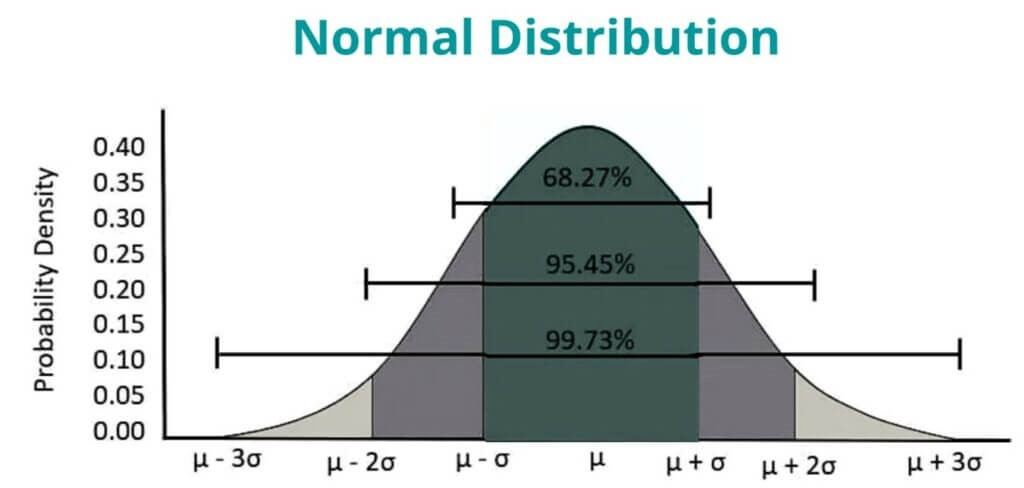
\includegraphics[width= 0.9\textwidth]{images/Normal-Distribution-1-1024x556.jpg}
    	\caption [Normal Distribution]{Normal Distribution \protect\cite{Normal}}  
    	\label{fig:Guassian Distribution}
\end{figure}


In data science, clipping refers to the process of limiting the range of values in a data-set. This is typically done to remove outliers or to handle cases where the data has extreme values that may skew the results of an analysis. Clipping can be applied to both uni-variate (single variable) and multivariate (multiple variable) data-sets. The process of clipping involves setting a threshold, and any data points that fall outside of that threshold are replaced with the threshold value. This can be done by replacing all values below a certain minimum threshold with the minimum threshold value, and all values above a certain maximum threshold with the maximum threshold value. Clipping can be useful in situations where extreme values in the data can have a disproportionate impact on the results of an analysis, such as in statistical modeling or machine learning. It can also be used as a pre-processing step to improve the performance of algorithms that are sensitive to outliers. 

Compared to the Z-score or IQR method for removing outliers the clipping method appears to be more appropriate for the data-sets dealt with in this thesis. The values or parameters monitored in the LTT are usually defined by tolerance limits. These tolerance limits are defined in each QPP documents. Every electronic device has a tolerance range for it's operation. When the device operates under the tolerance range, upper tolerance and lower tolerance limits, the device is considered to be functional and the data from the device is considered valid. With passage of time the components in DUT will end up having wear \& tear due to constant exposure to varying levels of external factors like temperature, shock etc as well as changing modes of operations. These deterioration means there would be change in output values that will not lie in the desired tolerance ranges. This is called as drift and would also be discussed in the next chapter. 

Clipping is a good approach to analyse the data as it permits only values or data lying in the tolerance window. The data that lies inside this window is valid and hence suitable for arithmetical operations such as arithmetic mean. The clipping method can also be used as means to observe the drift. The drift could be observed in the way, where the no. of values the end up lying outside of the tolerance windows can be observed and then determined whether the device is undergoing aging or deterioration or not. 

Thus, a combination of clipping and arithmetic mean can thus help in reducing the data size as well as making the condensed data more meaningful for the end user to analyze. 
\newpage

\subsection{Compression Algorithms}

Data, in general, could mean any type of output. Anything ranging from images to texts, videos to signals, numbers to e-mails can be called as Data. With increase in development of technology in different domains, the quality of data has improved significantly. At the same time, the size of data has also increased proportionately. With this trend arose the demand to efficiently store data. For this purpose, several data compression techniques have been developed in various fields over the years. Data compression algorithms are methods used to reduce the size of data without losing important information. 

There are several types of data compression techniques that are in existence. Of those, here are some common and relevant types of techniques : 

\begin{itemize}


    \item \textbf{Lossless compression} : These algorithms are designed to compress data in such a way that the original data can be exactly reconstructed from the compressed data. Examples of lossless compression algorithms include:
    \begin{itemize}
        \item LZW
        \item Huffman coding
        \item Run-length encoding
        \item Arithmetic Encoding
    \end{itemize} 


    \item \textbf{Lossy compression} : These algorithms are designed to compress data by discarding some of the information that is considered less important. These algorithms are most commonly used in image and audio compression. Examples of lossy compression algorithms include:
    \begin{itemize}
        \item Discrete Cosine Transform (DCT)
        \item Fractal compression
        \item Transform coding
        \item Quantization
    \end{itemize} 

    
    \item \textbf{Dictionary-based compression}: These algorithms are based on the idea of replacing a sequence of data with a reference to a dictionary of common sequences.
    Some examples of the same are :
    \begin{itemize}
        \item LZ77
        \item LZ78
        \item LZW
        \item LZMA
    \end{itemize} 
    
\end{itemize}

Lossless compression is a method of compressing data in such a way that the original data can be recovered exactly from the compressed data, without any loss of information. Lossless compression is used in situations where it is important to maintain the integrity of the original data, such as in medical imaging, scientific data, and text documents. The most common lossless compression algorithms are based on statistical methods, such as Huffman coding and arithmetic coding, which use the frequency of occurrence of different symbols in the data to create a more efficient representation of the data. Run-length encoding (RLE) is a method of data compression that is used to represent a sequence of data where repeating values are replaced with a single value and a count. The basic idea behind RLE is to identify runs of repeating values, and represent them using a shorter notation. For example, if we have a sequence of data consisting of the values 1, 1, 1, 2, 2, 3, 3, 3, 3, we can represent this using RLE as "3x1, 2x2, 4x3". This method is commonly used for image compression, as it is effective for image data that contains large areas of solid color. For example, a large image of a blue sky would contain many pixels with the value of blue, and RLE can efficiently compress this data. Lossless data compression algorithms can be used to compress text, images, audio and video files. They are also used in file archiving, backups, and data storage.


Lossy compression is a method of data compression in which some of the original data is discarded in order to achieve a higher level of compression. The goal of lossy compression is to retain the most important information while discarding less important information. This type of compression is commonly used in image and audio compression, as well as in video compression. One of the most widely used examples of lossy compression is JPEG, which is used for compressing images. In JPEG, the image is divided into small blocks called macro-blocks and each block is transformed into the frequency domain using the Discrete Cosine Transform (DCT). The DCT coefficients are then quantized and encoded using Huffman coding, which discards the less important coefficients. This results in a smaller file size but with a loss of some of the original image information.In addition, video compression like h.264 and h.265 also use lossy compression technique to compress the video data, they will take advantage of the temporal and spatial correlation of video to remove the redundant data and keep the important information. Lossy compression is widely used in applications where storage space is limited, such as in mobile devices and in streaming media. 

Dictionary-based compression is a method of data compression that utilizes a predefined dictionary of words or phrases to compress a given input stream of data. The basic idea behind this method is that many natural language texts, as well as other types of data streams, contain repeating patterns or sequences of characters, which can be replaced by shorter codes that represent those patterns in the dictionary. One of the most well-known examples of dictionary-based compression is the Lempel-Ziv-Welch (LZW) algorithm, which is commonly used to compress text files, image files, and other types of data. The LZW algorithm works by building a dictionary of phrases that are encountered in the input data, and then replacing each phrase with a code that corresponds to its position in the dictionary. Another example of dictionary-based compression is the Burrows-Wheeler transform (BWT), which is used in the bzip2 and gzip compression utilities. BWT is used in the bzip2 and gzip compression utilities, which are commonly used to compress log files, text files, and other types of data. 

From the above descriptions, it is very clear that lossy compression is not a suitable approach for compression of the data-sets. Each sampled data-point is important in the sense that regardless of valid or invalid data, it is an indication of the state of DUT. The valid data-points could be compressed or condensed into smaller sets of data-points while the invalid data-points can be used to study the characteristics of the errors in the DUT. Using lossy compression could cause loss of data-points which could change the complete characteristic of the log-file or analysis performed by the end user. 
%\ref{datalog}
Dictionary-based compression from it's characteristics is a subset of lossless compression. However,the target area for dictionary-based compression is different to the data-sets being utilized in this thesis. Going back to chapter 2, there are two different types of log files that are generated by the test systems, i.e .blf files and .asc files. Dictionary based compression use file zipping as one of the methods for data compression. Since .blf files are files that are 100s of GB in size and consist of different types of data-sets, file zipping appears to be a possible solution. The .blf files contain different types of data related to CAN traffic and metadata about that traffic. Hence, it is a possibility that one single custom algorithm could not be implemented on .blf files and it might require different approaches. File zip is a plausible solution for reducing such complexity and hence worth consideration. 

Lossless compression is the technique that is of most interest in this study. As mentioned earlier, a compression technique that could achieve data reduction without loss of information in crucial to handle the data-sets studied in this thesis. Of all the compression techniques which achieve lossless compression, RLE Encoding or Run-length Encoding is a method that can achieve such a lossless compression. It encodes runs of repeated data elements into a single data elements and a count. The method works by scanning the input data and counting the number of consecutive occurrences of each data element. These counts are then encoded along with the data element in the compressed data stream. An example of the same has been already discussed above.     

The RLE encoding can be used for dealing with .asc files. The .asc files are also log files generated from test-systems like .blf files. However, instead of consisting of information of all types of data from the test system like .blf files, the .asc files are parameter based log files. They contain information about parameters like voltage, current, time, temperature etc. in them. Since, the files contain multiple sets of similar data, RLE encoding can be considered a feasible solution to compress files of such types. 

\newpage

\subsection{Processing}

Having understood possible methods to reduce the file size to achieve meaningful data compression, it is necessary to understand the type of processing that could occur on the these data-sets. Processing is an important aspect of handling the log files as it deals with fetching , segregating and compressing the data. There are two types of data processing methods that can be implemented on the test systems. 

1) \textbf{Real-time Processing}: It is a method of data processing where data is processed immediately as it is generated or received. This method is used in applications that require immediate processing, storage, and retrieval of data, such as financial transactions, stock trading, and medical equipment monitoring. Real-time processing is more complex than batch processing, as it requires the immediate processing and storage of data, as well as the ability to retrieve data quickly. The main advantage of real-time processing is that it provides prompt and up-to-date information, which is crucial in many time-sensitive applications.

As is known already, the test systems are controlled by CANoe. This means that data logs can be processed at source or at destination. 

The data-logs are generated from the logging blocks defined in CANoe and written in CAPL code. Real time processing in this context would mean that logging blocks be used as source and compression algorithm be written in CANoe using CAPL code for the data-logs. System variables play crucial role in real time processing because data is read and written onto them from the test systems. If a buffer system is created, then it is possible read and write data that is logged from the test system into the compression algorithm simultaneously. A buffer is a temporary storage area in computer memory that holds data waiting to be processed or data that has been processed but not yet stored in its final destination. Buffers play an important role in computer systems by allowing the smooth flow of data between different stages of processing, reducing the impact of differences in data processing rates, and ensuring that data is properly managed and protected during transfer. There are different types of buffers, including input buffers, output buffers, and data buffers, that serve different purposes depending on the system architecture and the type of data being processed. Some of the types of buffers that could be considered useful for this purpose are as follows:

\begin{itemize}
    \item \textbf{FIFO} : FIFO buffer operates like a queue where the oldest data is processed first and new data is added at the end. It's advantages include ease of use and simplicity in processing data, as well as being well-suited for real-time applications. However, it requires larger memory space and is less efficient for data manipulation operations.

    \item \textbf{Circular Buffer} : Circular buffer operates in a cyclic manner where the oldest data is overwritten when the buffer is full. It's advantages include efficient use of memory and well-suited for real-time applications. It's main disadvantage is the complexity of implementation.
\end{itemize}

A circular buffer, also known as a ring buffer, is a data structure that is commonly used in real-time systems for buffering data streams. It is implemented as an array that has a fixed size, and a read and write pointer. When the write pointer reaches the end of the array, it wraps around to the start of the array. This is a much more memory efficient approach to process the data in real time compared to the FIFO buffer approach. FIFO even though being a simpler approach of implementation, is a resource heavy approach since it waits for the complete buffer to be written, filled and old discarded before the new data could start writing into it. 

These buffer systems could be defined inside a CAPL code which fetches data from the logging block with help of system and environmental variables. This would ensure that the logging and compression occurs simultaneously. With the help of buffers, data from the sensors could be read in real-time, then filtered for validity and then passed on to final logging block. The result of this complete process would be a log file in .asc format for the user to analyse in the most compressed form. The advantage to this approach is that no temporary storage for log files is required on external computers. Test-systems or systems running CANoe should have necessary computing memory available to facilitate this since it's a real time resource heavy task.


2) \textbf{Batch Processing} : It is a method of data processing where data is accumulated over time and processed in a single group or batch. This method is commonly used for routine tasks such as billing, and accounting. The main advantage of batch processing is that it can handle large amounts of data efficiently, as all the data is processed at once. Another advantage is that it allows for better use of resources such as processing power and memory. However, batch processing can also be time-consuming, as data must be accumulated before it can be processed, and the processing time may be lengthy, especially for large amounts of data. It is more suitable for routine tasks that do not require immediate processing and retrieval of data. 

The batch processing method gives opportunity to use different tools to analyse the log-files and process them. The log files in the .asc \& .blf format are stored in the test laptops at the end of LTT. The .asc files can be opened by default on CANoe as well as external programs like MS Excel unlike .blf files which can be accessed exclusively using CANoe. Batch processing of .asc format files is hence possible using programs like MS Excel. Although .asc aren't natively supported by MS Excel, it is possible to open, read and edit them in MS Excel using MS Excel wizard. The wizard allows to set the format of the file which is quite similar in approach to reading a .csv file in excel and thus enables to read the .asc file in user readable format. Excel Macros are then used to set filters, highlight specific data and many other purposes for the test engineer to analyse the log files and understand the performance of the DUTs. It is possible to write a VBA script that would compress the corresponding by filtering, segregating, summarizing the datas in the log files and then saving the compressed file. 

Another approach is to use a software tool or language to perform the data compression on the stored .asc files. Python is a very promising tool that could help in achieving this goal. Python has various libraries that enable it interact with files of various data types. This is of primary importance because to process the files, it is important to be able to read and write on them. Apart from this feature, python has many in-built mathematical functions pre-defined such as mean, variance etc. Python is also a very handy tool in dealing with MS-Excel files of .xls* formats. This is also crucial as python could be utilised as a method to convert .asc files into easy to access .xls* format files after performing data compression. Since python is a very robust and user-friendly tool, it is also possible to perform various types of analysis on the final log data or compressed data if ever needed by the engineer. 
\newpage
\subsection{QFD}

Quality Function Deployment (QFD) is a comprehensive approach to product development that involves a team of stakeholders working together to identify customer needs and create a product or service that meets or exceeds those requirements. It is a customer-focused methodology that aims to ensure customer satisfaction by designing a product or service that addresses customer needs and wants. One of the key advantages of QFD is that it helps to ensure that customer needs are understood and addressed early in the product development process. By involving customers and other stakeholders in the design process, QFD helps to ensure that the final product meets their needs and expectations. Additionally, QFD helps to improve the product development process by identifying areas where improvements are needed and by evaluating the trade-offs between different options or alternatives.

QFD is often used in manufacturing, service, and healthcare industries. It can be used for developing new products or services, as well as for improving existing ones. It is also used in quality management and process improvement. A short example of QFD in action is a car manufacturing company that wants to improve customer satisfaction with their vehicles. In this case, the car company would use QFD to gather customer feedback and identify customer requirements, such as fuel efficiency, safety features, and comfort. Next, they would use QFD to develop product characteristics, such as engine size and weight, and evaluate trade-offs between different options or alternatives. Finally, they would use this information to improve their existing vehicles and develop new ones that meet or exceed customer requirements.

QFD differs from similar approaches in that it is a customer-focused methodology that aims to ensure customer satisfaction by designing a product or service that addresses customer needs and wants. Additionally, QFD is a comprehensive approach that involves multiple stages, including the identification of customer needs, the development of product characteristics, and the evaluation of trade-offs between different options or alternatives.

There are five different approaches that can be derived from the study of different methods for compression from the sub-chapters above. These are as follows : 

\begin{itemize}
    \item Data compression via mathematical reduction in real-time processing : The algorithm is implemented on CANoe platform with the clipping and arithmetic mean to reduce the size of final log data.

    \item Data compression via mathematical reduction in batch processing : The algorithm is implemented via Python as post processing method with clipping and arithmetic mean to reduce the size of existing logged data.

    \item Data compression via byte size reduction in real-time processing : Run Length Encoding algorithm is implemented on CANoe to reduce the size of the log file.

    \item Data compression via byte size reduction in batch processing : Run Length Encoding algorithm is implemented on existing log files via Python.

    \item Data compression via mathematical reduction through a combination of real-time and batch processing : This is a combination of two processing methods so that reduction can be processed in real-time on CANoe system and then using the python to perform analysis on the reduced data
\end{itemize}


\subsubsection{Pairwise comparison \& Weighted Analysis} 

Pairwise Comparison is a decision-making technique used to compare and rank items based on their relative importance, priority or weight. It is a systematic method that is used in several fields such as software engineering, project management, operations research and decision theory. The aim of pairwise comparison is to determine which of two items is preferred or considered more important, or to rank a set of items in order of importance.

In pairwise comparison, each item is compared with every other item, and the results are recorded in a matrix. This matrix is used to compute the relative importance of each item. Pairwise comparison is used to quantify the relative strength of relationships between two items, which can then be used to rank them. For example, in software engineering, pairwise comparison can be used to rank requirements, in order to determine which ones are most important and should receive priority in development.

One of the advantages of pairwise comparison is that it provides a simple and systematic way to rank items, and it can be used to compare items with different attributes. The approach is highly flexible and can be adapted to a variety of decision-making situations. It is particularly useful when there is no clear objective method of comparison, or when the items being compared are subjective in nature.

Another advantage is that pairwise comparison is easy to understand and can be performed by people with a wide range of knowledge and expertise. It is also less time-consuming and less expensive than other methods, such as multi-attribute decision-making methods, which require more data collection and analysis.

Before performing pairwise comparison it is important to list the requirements that are analysed by this method : 

\begin{itemize}
    \item Compression factor 
    \item User friendliness  
    \item Data evaluation capability 
    \item Troubleshooting friendly 
    \item Multi-format support 
    \item Extensibility  
    \item Data re-usability 
    \item Additional resources
    \item Execution time
\end{itemize}

This thesis studies two types of log files : .asc and .blf files. For the .asc files there are multiple options for achieving data compression since .asc file is not platform restricted. It is possible to access .asc files even without CANoe software. Moreover, they are configurable log file in the sense, it can be set via CANoe - CAPL what parameters should be logged into .asc files. Since the type of data occurring in a .asc file is already and the file is always open for access it is possible to perform data compression on these files using different approaches. 

However, the same cannot be said in the case of .blf files. The .blf file are inaccessible without CANoe platform. This makes it inaccessible to 3 out of 5 data compression methods discussed above which include both the batch processing methods and the third method being the combination of real-time and batch processing method. This leaves the .blf files to be compressed by remaining methods of real-time processing : 1) Mathematical Reduction 2) Byte Size Reduction. The contents of .blf files are in binary format and they contain all types of messages on CAN bus. Since .blf files are in binary format it is not possible to implement the arithmetic mean reduction method as it applies to only integer type data. The sole compression method left out of the bunch is the Byte size reduction method. It was earlier discussed that RLE would be a suitable method for performing byte size reduction, however, that was in context of .asc files. RLE works by identifying runs of consecutive data elements and representing them using a single data element and a count of number of consecutive elements. Given the complexity of data-sets in .blf files, implementing RLE encoding on such files would not be feasible and not in the scope of this thesis. However, there is another encoding method that could replace RLE for .blf files and achieve data compression. This method has been discussed earlier which is the file zip method. File zipping is a process that can be achieved with various compression techniques like LZW, LZMA, LZ77 etc. The rate of compression achieved by zipping a blf file is discussed in the next chapter. However, at this juncture it can be said there is no effective method to compress the size of .blf file than what already exists in the form of file zipping software. Henceforth, for every study and implementation only .asc files will be considered when log files are mentioned. The pairwise comparison and weighted analysis of log files would also be performed only on the .asc files. 

The following image shows the pairwise comparison of all the requirements mentioned above for the log files. \newpage


\begin{figure}[!h]
    	\centering
    	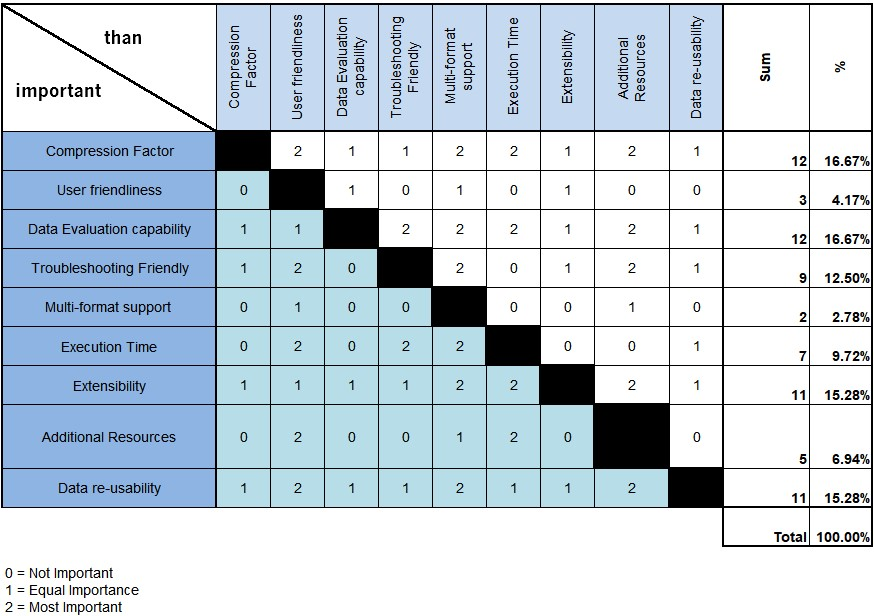
\includegraphics[width= 0.9\textwidth]{images/Paarweise.jpg}
    	\caption [Pairwise Comparison]{Pairwise Comparison}  
    	\label{fig:Pairwise Comparison}
\end{figure}

In the above figure, the pairwise comparison is conducted to determine the weightage of the requirements. This method enables the user to determine the priority of requirements for product development. As shown in the figure, the requirements are compared with each other and a 3 step priority marker is used to aid this comparison. 0 ,1 and 2 are the three indicators of priority with increasing priority compared with each other. Consider, the row Compression Factor where it is compared with 8 other requirements to determine it's weightage. Compression Factor is determined to be more important than the following factors : 1) User Friendliness 2) Multi-Format Support 3) Execution Time 4) Additional Resources. Whereas compared to the following requirements : 1) Data Evaluation Capability 2) Troubleshooting Friendly 3) Extensibility 4) Data Re-usability , the requirement Compression Factor is given equal importance. This is very intuitive and easy to understand in the sense that the key feature of a Data compression algorithm which is Compression Factor is given more importance over factors like User Friendliness, Multi file support, Execution Time and Additional Resources.

Any of the above four requirements can be compromised or rather given a lower priority of execution in order to achieve better compression rate. For e.g the outcome of the pairwise comparison will help determine an algorithm for data compression of .asc files. It might not be feasible to develop an algorithm that could achieve best compression for both .blf and .asc file types. Since, it is already determined that .blf files have very limited flexibility in terms of application of a data compression algorithm on it, priority could be given to the compression factor as a requirement and an algorithm could be selected which provides the highest compression for .asc files. Thus a higher importance is given to Compression Factor than to Multi format support. Similar parallels could be drawn to Compression Factor vs Execution time , Compression Factor vs Additional resources etc.

At the end of pairwise comparison compression factor and data evaluation capability achieve highest priority amongst all requirements, which is validated by the goal of this thesis. Extensibility or expand-ability of the algorithm and Data re-usability ,i.e ability to make use of values post compression, come close second. The percentage column is of great significance here. Until now, the pairwise comparison was used to determine which requirements should be assigned higher priority in product development cycle. Once the priorities of each requirements are determined, the next step is determine which algorithm is valid and imbibes the result of the pairwise comparison in itself. Weighted Analysis of algorithms helps in achieving this goal. The percentage column derived from pairwise comparison is also a metric which can be used in the weighted analysis. At the end of weighted analysis comparison, one out of five algorithms would be selected which is the closest to fulfilling all the requirements set in this thesis. 

\begin{figure}[!h]
    	\centering
    	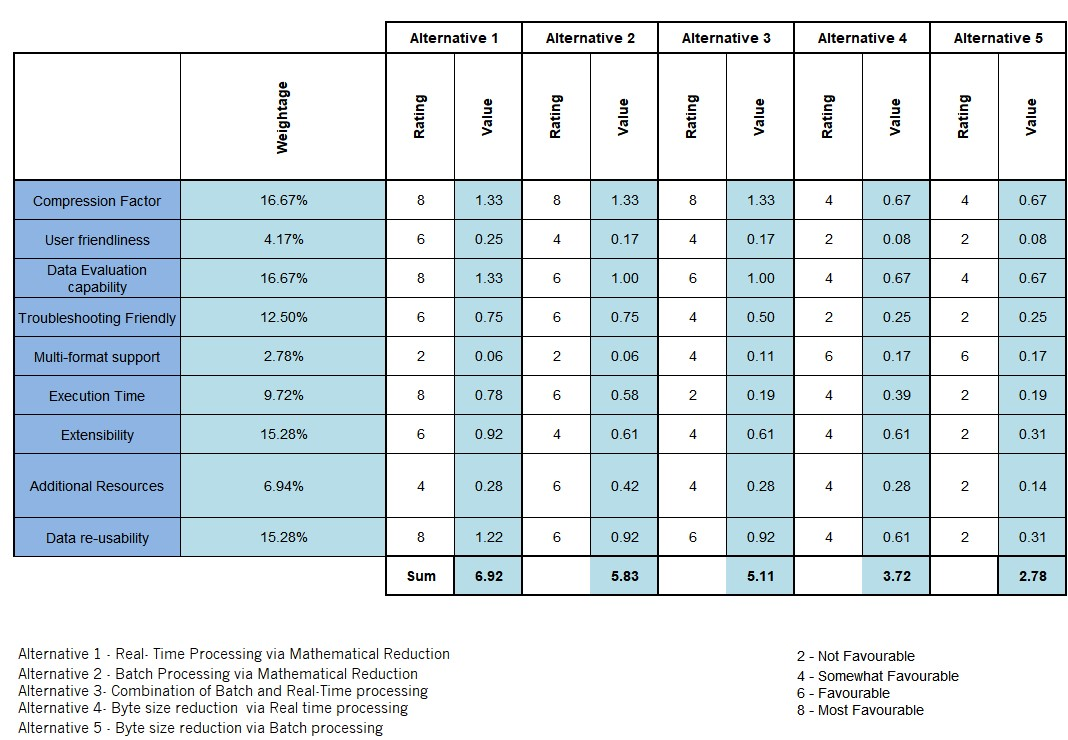
\includegraphics[width= 1\textwidth]{images/Weighted Analysis.jpg}
    	\caption [Weighted Analysis]{Weighted analysis}  
    	\label{fig:Weighted Analysis}
\end{figure}

The above diagram indicates the weighted analysis of all the 5 possible algorithms to achieve data compression on .asc files. The 5 algorithms are described as 5 alternatives in the above diagram. Compared to pairwise comparison, the rating, here, is not done on basis of priority instead the rating is symbolic of the property of the algorithm. There are 4 levels of Rating selected for each algorithms: from 2 all the way to 8. 2 is the least favourable rating which indicates that a particular requirement is not fulfilled by the algorithm. Whereas 8 indicates most favourable rating which indicates that for a particular requirement, the algorithm is the best fit. The following formula is used to calculate the weighted value assigned to each requirement fulfilling capability of the algorithm :
\begin{equation}
 Value (V)  = Weightage * Rating
\end{equation}
The Sum is the summation of all the weighted values : $\Sigma(Vn)$ . 

Each algorithm has it's own unique characteristics and the weighted analysis is a great method to showcase it's uniqueness. For example, alternative 1, 2 \& 3 all use the same mathematical model of arithmetic mean combined with filtering to achieve compression hence they have similar ratings for compression factor. However, there is a stark contrast in the three alternative when looking at a feature like execution time. Alternative 1 involves real time processing, hence the total execution time, calculated from test start to generation of reduced log file, is the lowest. Alternative 2 needs log files to be generated in order to perform compression in post processing approach, hence the execution time is increased in comparison to alternative 1. Alternative 3 uses a combination of both the alternative 1 \& 2, hence the total execution is greater than alternative 1 and 2. Thus, alternative 3 is the least suitable from the perspective of execution time as a key feature of the algorithm. 

At the end of weighted analysis, the algorithm with highest valuation wins. This means that the algorithm with the highest valuation is the most appropriate suit for all the defined requirements. As per \ref{fig:Weighted Analysis}, the alternative 1 has the highest valuation followed by alternative 2. The alternatives 4 and 5 have received the least valuations owing to various unsuitable factors such as :

\begin{itemize}
    \item Low compression factor : compared to mathematical model byte size reduction method is not very robust as it is heavily dependent on repetition of values
    \item User friendliness : complexity of the algorithm design and execution makes it unfavourable for the end user to use it intuitively
    \item Data evaluation capability : Due to encoding method used to implement these algorithms, it is possible data re-usability is drastically reduced which would in turn make data evaluation difficult
\end{itemize}

The sole feature where alternative 4 \& 5 outshine the other three alternatives are it's support for multi format file support. It is, theoretically, possible to implement these algorithms on both .asc and .blf files. However, the complexity that accompanies with practically implementing these methods outweighs the benefits they provide by offering multi file support. 


Hence, at the end of this study, it can be concluded that a mathematical reduction method accompanied with filtering or clipping is the most suitable approach for reducing the data-sets concerned with this thesis. The approach of real-time processing along-with mathematical reduction provides the best possible compression algorithm. Every scientific approach requires alternatives in case the most suitable approach hits a bottleneck due to unforeseen scenarios. In such scenarios, batch processing along-with mathematical reduction is a relevant alternative coming close second in the weighted analysis study of all the algorithms. 